%!TEX root = ../thesis.tex
In this section we are going to cover our evaluation of our \emph{textile touch} explorative prototype, more specifically this is the latest prototype covered in \ref{ch:textiletouch:it3}~(\nameref{ch:textiletouch:it3}).
We have two primary goals of this evaluation.
On the one hand, we want to evaluate on the interaction potentials of using simple gestures as input control.
This goal involves using the prototype as an interactive device to control existing devices of the home.
On the other hand, we want to explore our prototype in alternative contexts.
This goal should shed light on the prototypes potential of encouraging alternative usages than controlling existing devices.

Evaluations were done over \todo{three} rounds to get a diversity in age groups of the test participants.
We were interested in shedding light on the diversity of creative ideas a child would bring compared to and adult.

\todo{mere + afrunding}
\blank
As mentioned earlier in \emph{ \nameref{ch:textiletouch:it3} } we have developed a simple audio and video application which mimics some of the functionality of a television and a stereo system.
This application was used as the starting point for evaluating the value of using the prototype for controlling existing devices.
During evaluation we would connect the prototype setup and computer to the home TV to resemble the real situation and the prototype would for instance be layn as part a of sofa, as a table cloth or attached to a wall as for example wallpaper.
From there on the basics of interaction were understood and further discussions and explorations could be made extending beyond the limits of the audio/video application.

Moving on from looking at the potentials of controlling existing devices of the home, the evaluations would take a more discussion-oriented direction where alternative usages and activities were the primary focus.
To start off discussions we would present some of our own ideas of potential usages.
\todo{mere}
\blank
An overall note to be taken from the evaluations was that the participants found it intriguing to try out the prototype.
Not so much for the purpose of the simple test application, but more for the idea of interacting with textile and using it for digital input.
Surely they are accustomed to using touch interaction on the small surfaces of everyday consumer devices such as displays and touchpads, but not with inherently non-electronic materials such as textile. \todo{lidt mere generelt her}
\blank
In the following two sections we highlight some of the findings of the evaluations.

\subsection{The concept as a controller for existing devices}
\todo{\dots}
\blank

The idea of a pulsating vibration during touch was well received as an indication of touch being recorded and to delimit for example the digital sofa from the physical sofa. \todo{what?}
As we anticipated, the haptic feedback got some critique and it was pointed out that it should give a stronger sensation.
We had placed the vibration motor in the center beneath the prototype and vibrations were therefore only noticeable in that area.
With a less powerful motor the subtle touch sensation of ones hand against the texture of the linen could easily drown the vibrations as well.

A concern brought up by several participants was that there was a lack of indication of the stroke one had just applied.
A promising visual feedback technique for display-oriented interaction was suggested by one of the participants.
The idea was to get real-time feedback on a display when providing touch input by seeing the strokes made as an overlay on the display.
In figure~\ref{fig:textiletouch:eval:overlay} we have made an example where two semi-transparent strokes are overlaying a TV programme. 

\begin{verbatim}
taler til det indre dovendyr
   rette paa gardiner
uoverenstemmelser mellem handling og konsekvens
skal i hvert fald ikke blive et komplekst nyt sprog man skal laere
   ensartet interaktion paa tvaers af applikationer
\end{verbatim}

\begin{figure}[h]
	\centering
  		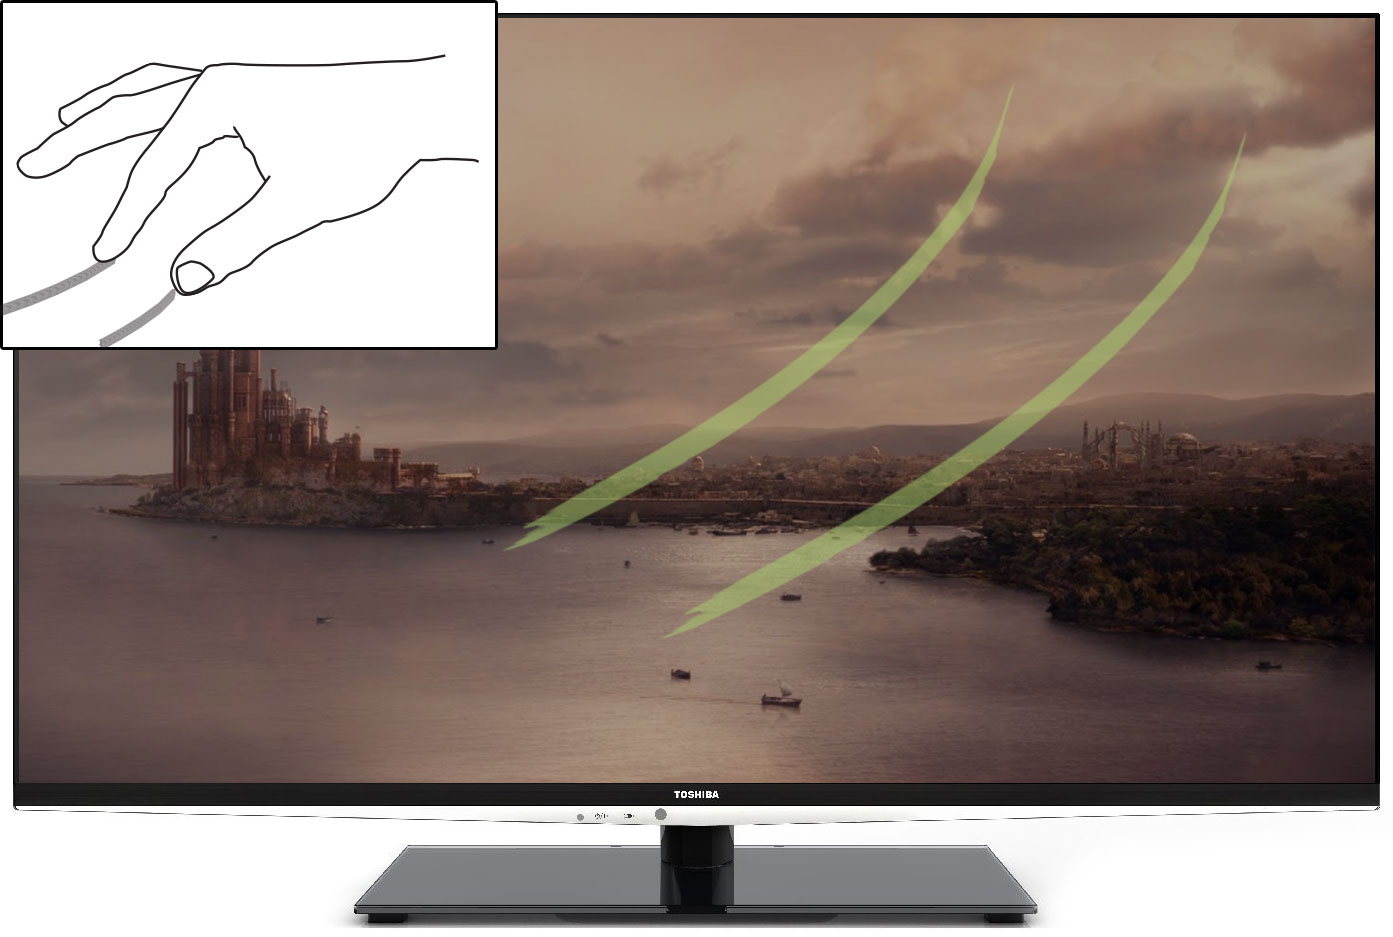
\includegraphics[width=3in]{figures/touch/evaluation/gesture_overlay}
	\caption[Gesture input as an overlay for real-time feedback.]
   {Gesture input as an overlay for real-time feedback.}
   \label{fig:textiletouch:eval:overlay}
\end{figure}

\subsection{Potentials of alternative usages}

\begin{verbatim}
**** Paw + Morten ****
* tegning paa overflader: "hvis danmark nu er her ... og holland her, saa ..." 
	- for at forklare ting.
* boernevaerelse - legemaatte, hvor foraeldre kan se aktivitetsniveau for 
	deres unger og dermed ikke behoever at tjekke op paa dem hele tiden.
* sleep cycle taepper
* handikaphjem
	* vildt mange ting der skal styres
    * mobilitet er begraenset
* aeldrehjem
    * crash taeppe - folk med parkison der ofte vaelter eller lign.
        * eller alle flader
    * "hvis man ikke har noget paa kan det ikke tages" - nuvaerende situation 
		hvor aeldre faar "halsbaand" (falde-detektor) paa, som de tager af i tide og utide.
* Sikkerhed. Den usynlig noegle - man skal vide hvor man input delen er for 
	at kunne lave en "adgangsgestik".
    * Eller det, at mennesker har en unik "haandskrift" der kan anvendes 
		paa touch overfladen.
    * doermaatte
\end{verbatim}



\subsection{Future work}
\label{ch:textiletouch:futurework}

There are several points about the prototype that are candidates for future work.
We do see the prototyp

On the technical side there is room for improvement.
As the technology allows for multi-touch input it would be a great improvement for the user experience.
Multi-touch provides a much richer interaction style \todo{reference?} compared to single-touch and has become a standard in modern smart phone displays and laptop touchpads, most notably for scrolling, zooming and rotation.
The gesture recognition framework used for the prototype, \$P, will work just fine with multi-touch and will not require further adjustment as the method of input is totally decoupled from the recognition framework. \todo{though gestures or symbols are not the same as real-time gestures on a mouse-pad such as zooming}
Instead it is our peak detection algorithms that need to be reimplemented and take multiple peaks in to account.
Figure~\todo{ref} shows a frame of input where several peaks made by finger inputs are detected. \todo{provide reason for not implementing multi-touch in the firstplace?}

As can be seen in the figure every peak is surrounded by some noise created by finger pressure propagating away from the peak spot.
It should be noted that we do not consider values in the immediate proximity of a peak to be noise as we use these values to make interpolation and thereby scale the resolution by a factor a 10.
We have already taken steps to reduce this by implementing a simple averaging filter in the software 
where a sample is an average of \emph{x} previous samples.
There are also steps to be taken on the hardware side where a noise filter could reduce the signal-to-noise ratio before entering the software part.


Mechanisms for providing direct feedback on the textile surface should be further investigated.
Vibrations \todo{\dots}

\todo{ting der er belyst fra evaluering \dots}

\begin{verbatim}
dette er ikke faerdig prototype - snakke om forskellige retninger
\end{verbatim}

